Paragraph introducing the topics covered in this section. Points to hit:
\begin{itemize}
    \item 
\end{itemize}


% The aim of the first half of this thesis is to understand how the Chern number -- which is well-defined only for non-interacting quantum systems with translational symmetry -- can be extended to disordered materials. 

% There are three parts, first we introduce the concepts of Berry phase and Chern number, discussing the ways that they can be used to classify non-interacting quantum systems with no symmetries. Next we define the Qi-Wu-Zhang model, which provides a simple example of a Chern insulator on a square lattice. 

\section{Abelian Berry Phase and the Chern Number} \label{sec:Abelian Berry Phase and the Chern Number}

In this section we present a careful discussion of Berry's phase, Berry curvature and the Chern number \cite{berry_quantal_1984,avron_homotopy_1983}, showing how these quantities may be calculated form the band structure of a general non-interacting insulator. There are two cases to discuss: for a finite system the Brillouin zone constitutes a discrete lattice of states. Thus, in \textsection\ref{sec:discrete_berry}, we show that Berry phase can be understood as the relative phase between adjacent states, and that Berry flux is defined on the plaquettes of the lattice. In \textsection\ref{sec:continuous_berry} we consider the case of an infinite system. There the Brillouin zone is a continuous manifold and the band structure defines a mapping from this manifold to the Hilbert space of periodic states. In this case, Berry's phase is a geometric property of this smooth mapping. In both cases, we derive the form of the Chern number and justify its quantisation. Finally, in \textsection\ref{sec:an_example} we provide an example -- that of a two level system -- where the Berry flux can be understood straightforwardly in terms of the flux emitted by a monopole, allowing us to present a simple visual argument for the quantisation of the Chern number. Our discussion will largely follow \cite{asboth_berry_2016,resta_geometry_2020}.

\subsection{A Discrete Brillouin Zone} \label{sec:discrete_berry}

In quantum mechanics a state is defined as an equivalence class of vectors, where two states that differ only by a complex phase are considered physically equivalent,
\begin{align}
    \ket{\psi} \sim e^{-i\alpha}\ket{\psi}.
\end{align}
Thus, we have a redundancy built into our description of physics. This means that one can define a gauge transformation -- multiplying a state with a complex phase, a $U(1)$ gauge -- that is guaranteed not to affect the state in any measurable way. Any derived quantity must be invariant under gauge transformations to qualify as a physical observable.

Now, let us consider an arbitrary set of states in the same Hilbert space, $\{ \ket{\psi_j}\}$. Analogous to the `global' gauge transformation presented above, we may define a `local' gauge transformation here, where we apply a different phase to each individual state,
\begin{align}
    \ket{\psi_j} \rightarrow e^{-i\alpha_j}\ket{\psi_j}.
\end{align}
Again, the physical meaning of each state is unaffected, so all observable quantities must be invariant under this transformation. Thus, one might wonder whether any \textit{phase-like} quantity calculated from these states can have a physical meaning. For example, the relative phase between state $j$ and $k$, $\gamma_{j,k}$ can be defined as
\begin{align}
    e^{-i\gamma_{j,k}} = \frac{\braket{\psi_j|\psi_k}}{|\braket{\psi_j|\psi_k}|}.
\end{align}
Clearly this quantity is invariant under a global gauge transformation, however it is not invariant under a local transformation, changing according to
\begin{align}
    e^{-i\gamma_{j,k}} \rightarrow e^{-i(\gamma_{j,k}+\alpha_j - \alpha_k)},
\end{align}
and so cannot be a physical observable. In order to construct a gauge-invariant object, let's pick a set of $n$ ($\geq 3$) states $\ket{\psi_j}$ and arrange them in a loop.
\begin{center}
    \begin{tikzpicture}

\def  \angoff {20}
\def \picsize {1.8}
\def \edistance {0.5}
\def \anground {72}

\draw [-latex,domain = \angoff:\anground-\angoff] plot ({\picsize * cos (\x + 90)}, {\picsize * sin (\x + 90)});
\draw [-latex,domain = \angoff:\anground-\angoff] plot ({\picsize * cos (\x + 90+\anground)}, {\picsize * sin (\x + 90+\anground)});
\draw [-latex,domain = \angoff:\anground-\angoff] plot ({\picsize * cos (\x + 90+2*\anground)}, {\picsize * sin (\x + 90+2*\anground)});
\draw [-latex,domain = \angoff:\anground-\angoff] plot ({\picsize * cos (\x + 90+3*\anground)}, {\picsize * sin (\x + 90+3*\anground)});
\draw [-latex,domain = \angoff:\anground-\angoff] plot ({\picsize * cos (\x + 90+4*\anground)}, {\picsize * sin (\x + 90+4*\anground)});

\draw node at (90:\picsize) {$\ket{\psi_1}$};
\draw node at (90+\anground:\picsize) {$\ket{\psi_2}$};
\draw node at (90+2*\anground:\picsize) {$\ket{\psi_3}$};
\draw node at (90+3*\anground:\picsize) {$...$};
\draw node at (90+4*\anground:\picsize) {$\ket{\psi_n}$};

\draw node at (90+0.5*\anground:\picsize+\edistance) {$e^{-i \gamma_{1,2}}$};
\draw node at (90+1.5*\anground:\picsize+\edistance) {$e^{-i \gamma_{2,3}}$};
\draw node at (90+4.5*\anground:\picsize+\edistance) {$e^{-i \gamma_{N,1}}$};

\end{tikzpicture}
\end{center}
We can now define a new quantity, the Berry phase, as
\begin{align}
    e^{-i \gamma_{B}} = \frac{\braket{\psi_1|\psi_2}\braket{\psi_2|\psi_3}...\braket{\psi_N|\psi_1}}{|\braket{\psi_1|\psi_2}\braket{\psi_2|\psi_3}...\braket{\psi_N|\psi_1}|}
\end{align}
Another way of writing this would be
\begin{align}  
    \gamma_{B} = -\arg \tr 
    \left [ \hat\psi_{1} \hat\psi_{2} 
    \, ... \,
    \hat\psi_{N} \right ],
\end{align}
where the trace is over the whole system, and $\hat \psi$ is shorthand for the density operator
\begin{align}
    \hat \psi_{i} = \ket{\psi_{i}}\bra{\psi_{i}}.
\end{align}
This quantity is clearly gauge-invariant, since any phase applied to a state $\ket{\psi_m}$ will show up twice, once from $\braket{\psi_m|\psi_{m+1}}$ and once from $\braket{\psi_{m-1}|\psi_{m}}$. The phase will have opposite sign in each of these expressions, so they cancel out. Furthermore, we can see that the Berry phase around a loop is simply the sum of all the relative phases around that loop modulo $2\pi$.
\begin{align}\label{eqn:discrete_berry_sum}
	\gamma_B = \sum_{n=1}^N \gamma_{n,n+1} \mod 2\pi
\end{align}


\subsubsection{Berry Flux}

Now suppose that we have a large number of states arranged in a 2D grid. These states  $\ket{\psi_{\textbf k}}$ are labelled with a pair of indices $k_x$ and $k_y$. In general, this parameter $\textbf k$ will refer to the crystal momentum, however the construction is equally valid for any other parameter that defines a 2D grid of quantum states, shown in Fig.~\ref{fig:berry_grid}.

\begin{figure}
    \begin{center}
        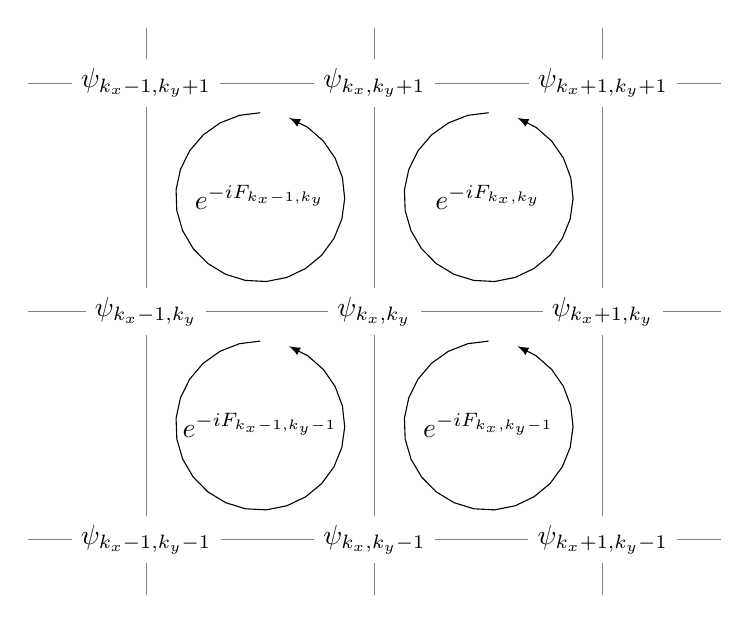
\begin{tikzpicture}

\def \gridsize{2.9}

\draw[step=\gridsize cm, help lines] (-\gridsize-1.5,-\gridsize-0.7) grid (\gridsize+1.5,\gridsize+0.7);
\draw node [fill= white] at (0,0) {$\ket{\psi_{k_x,k_y}}$};
\draw node [fill= white] at (\gridsize,0) {$\ket{\psi_{k_x+1,k_y}}$};
\draw node [fill= white] at (\gridsize,\gridsize) {$\ket{\psi_{k_x+1,k_y+1}}$};
\draw node [fill= white] at (0,\gridsize) {$\ket{\psi_{k_x,k_y+1}}$};
\draw node [fill= white] at (-\gridsize,0) {$\ket{\psi_{k_x-1,k_y}}$};
\draw node [fill= white] at (0,-\gridsize) {$\ket{\psi_{k_x,k_y-1}}$};
\draw node [fill= white] at (-\gridsize,-\gridsize) {$\ket{\psi_{k_x-1,k_y-1}}$};
\draw node [fill= white] at (\gridsize,-\gridsize) {$\ket{\psi_{k_x+1,k_y-1}}$};
\draw node [fill= white] at (-\gridsize,\gridsize) {$\ket{\psi_{k_x-1,k_y+1}}$};

\draw [-latex, domain = 0:340] plot ({0.37 *\gridsize* cos (\x + 90) + 0.5 * \gridsize }, {0.37 *\gridsize* sin (\x + 90) + 0.5 *\gridsize });
\draw [-latex, domain = 0:340] plot ({0.37 *\gridsize* cos (\x + 90) - 0.5 * \gridsize }, {0.37 *\gridsize* sin (\x + 90) + 0.5 *\gridsize });
\draw [-latex, domain = 0:340] plot ({0.37 *\gridsize* cos (\x + 90) + 0.5 * \gridsize }, {0.37 *\gridsize* sin (\x + 90) - 0.5 *\gridsize });
\draw [-latex, domain = 0:340] plot ({0.37 *\gridsize* cos (\x + 90) - 0.5 * \gridsize }, {0.37 *\gridsize* sin (\x + 90) - 0.5 *\gridsize });

\draw node at (0.5*\gridsize, 0.5*\gridsize) {$e^{-i F_{k_x,k_y}}$};
\draw node at (0.5*\gridsize, -0.5*\gridsize) {$e^{-i F_{k_x,k_y-1}}$};
\draw node at (-0.5*\gridsize, 0.5*\gridsize) {$e^{-i F_{k_x-1,k_y}}$};
\draw node at (-0.5*\gridsize, -0.5*\gridsize) {$e^{-i F_{k_x-1,k_y-1}}$};

\end{tikzpicture}
    \caption[A grid of states parametrised by a discrete parameter. ]{A grid of states parametrised by the discrete variables $\textbf k$, given by $\ket{\psi_{k_x,k_y}}$. For each plaquette, the Berry phase is calculated by taking the inner products of the states going counterclockwise around the loop.}
    \label{fig:berry_grid}
    \end{center}
\end{figure}%

We introduce a new quantity called the Berry flux, defined as the Berry phase around a plaquette on the grid,
\begin{align}\label{eqn:berry_flux}
    F_{\textbf k} =  
    - \arg \tr \left [ 
        \hat \psi_{k_x,k_y}
        \hat \psi_{k_x+1,k_y}
        \hat \psi_{k_x+1,k_y+1}
        \hat \psi_{k_x,k_y+1} 
        \right ].
\end{align}
$F_{\textbf k}$ is just the sum (mod $2\pi$) of the relative phases along each edge of the plaquette starting at point $\textbf k$. Thus, the Berry phase around some arbitrary loop can be written as a sum of the Berry flux for all plaquettes encircled by the loop. In this sum, the phase along any internal edge appears with opposite sign in the values of $F_{\textbf k}$ for the two adjacent plaquettes, leaving only the phase along the boundary,
\begin{align} \label{eqn:berry_sum_discrete}
    \exp 
    \bigg [
        -i \sum_{\substack{\textup{inside} \\ \textup{region}}}F
    \bigg ] 
    = \exp \bigg [ 
        -i\sum_{\textup{boundary}} \gamma
    \bigg ]
\end{align}
This resembles Stokes' law, however there is a subtlety worth mentioning. All we have required is that the complex exponential of each sum is the same. This does \textbf{not} mean that the sum of the Berry flux inside a region is equal to the sum of relative phases around the boundary, since they are allowed to differ by an arbitrary multiple of $2\pi$.


\subsubsection{Chern Number} \label{sec:discrete_chern}
Now let's assume that our grid of $\textbf k$ points has periodic boundaries -- as is the case for states on the Brillouin zone -- with $1\leq k_x \leq N_x$ and $1 \leq k_y \leq N_y$. The lattice is a discretisation of the torus -- a closed manifold. Thus, let us ask what the total flux through the whole manifold is. Following the argument of Eqn.~\ref{eqn:berry_sum_discrete}, the total Berry flux must satisfy 
\begin{align}\label{torus_sum}
    \prod_{k_x=1}^{N_x}\prod_{k_y=1}^{N_y}e^{-i F_{k_x,k_y}} = 1,
\end{align}
because every edge in this sum is an internal edge, and thus they cancel out. As before, this does not mean that the sum of all Berry fluxes in the system vanishes, rather the sum must be a multiple of $2\pi$. Thus let us define this multiple as the Chern number, $\mathcal Q$,
\begin{align}\label{eqn:discrete_chern_number}
    \mathcal Q = \frac{1}{2\pi} \sum_{k_x,k_y}F_{k_x,k_y}.
\end{align}
$\mathcal Q$ is necessarily restricted to integer values, since a non-integer value would contradict equation \ref{torus_sum}.

\subsection{Topology of a General Hamiltonian}\label{sec:continuous_berry}

Now let us consider the case of a smooth parameter space. We start by defining some arbitrary Hamiltonian $H(\textbf R)$, which depends on some smooth parameter $\textbf R \in \mathcal R$. For every value of $\textbf R$, the Hamiltonian has eigenstates $\ket{\psi_n (\textbf R)}$ with corresponding energies $\varepsilon_n$. As before, these eigenstates are only well-defined up to a global phase. Thus, let consider a single state $\ket{\psi(\textbf R)}$ and define a local gauge transformation, applying an $\textbf R$-dependent phase $\alpha(\textbf R)$ to all the states over this band.
\begin{align}
	\ket{\psi(\textbf R)} \rightarrow e^{-i\alpha(\textbf R)}\ket{\psi(\textbf R)}.
\end{align}
Before we continue, let us define a \textit{smooth gauge} as a choice of gauge that ensures that the $\textbf R$-derivative of a state, $\nabla_{\textbf R}\ket{\psi(\textbf R)}$ is always well-defined -- that is, $\alpha(\textbf R)$ does not change discontinuously. In general, it is not always possible to pick a gauge that is globally smooth over all of $\mathcal{R}$, however it \textit{is} always possible to pick a locally smooth gauge around the neighbourhood of a given point in $\mathcal{R}$.

In analogy to the relative phase in the previous section, let us quantify phase between a state at $\textbf R$ and a state that is infinitesimally displaced from it, at $\textbf R + d \textbf R$,
\begin{align}
    e^{-i\Delta\gamma} = \frac{\braket{\psi(\textbf R)|\psi(\textbf R+d\textbf R)}}{|\braket{\psi(\textbf R)|\psi(\textbf R+d\textbf R)}|}.
\end{align}
Taking the limit of small $d\textbf R$ we can express $\ket{\psi(\textbf R+d\textbf R)}$ to first order in $d\textbf R$ as
\begin{align}
    \ket{\psi(\textbf R+d\textbf R)} = \ket{\psi(\textbf R)} + d\textbf R \cdot \nabla_{\textbf R} \ket{\psi(\textbf R)}.
\end{align}
Which means that
\begin{align}
    \braket{\psi(\textbf R)|\psi(\textbf R+d\textbf R)} = 1 + \braket{\psi(\textbf R) | \nabla _{\textbf R}|\psi(\textbf R)}\cdot d\textbf R .
\end{align}
Now, noticing that $ \braket{\psi(\textbf R) | \nabla_{\textbf R} |\psi(\textbf R)}$ is pure imaginary, we can show that
\begin{align}\label{A_def}
    \Delta \gamma &= \textbf{A} \cdot d\textbf R, \\
    \textbf{A}(\textbf R)& = i
    \braket{\psi(\textbf R) | 
    \nabla_{\textbf R} |
    \psi(\textbf R)} . \label{eqn:cont_berry_connection}
\end{align}
The quantity multiplying $d\textbf R$ is the Berry connection $\textbf{A}(\textbf R)$. Like the relative phase in the previous section, it is not a gauge-invariant quantity. Under a gauge transformation it changes according to
\begin{align} \label{eqn:gauge}
    \textbf{A}(\textbf R) \rightarrow \textbf{A}(\textbf R) - \nabla _{\textbf R} \alpha(\textbf R)
\end{align}
Now let us suppose that we slowly transform our Hamiltonian around some closed path $\mathcal C$ in $\textbf R$-space and keep track of the phase picked up by a given state.\footnote{In \cite{berry_quantal_1984}, Berry originally proposed this transformation as an adiabatic process, where we modify the Hamiltonian extremely slowly, and many sources (e.g.~\cite{xiao_berry_2010}) propose the Berry phase in that framework. In that case, one has to do a little extra work to keep track of the energy-dependent phase that a state picks up $\sim e^{-i \varepsilon t}$ alongside the topological phase determined by $\textbf A$. Here we shall neglect this, only considering the \textit{instantaneous eigenstates} at different values of $\textbf R$. For a thorough explanation, see \cite{vanderbilt_berry_2018}.} In analogy with Eqn.~\ref{eqn:discrete_berry_sum}, the Berry connection allows us to calculate the total phase accumulated over this route, according to
\begin{align} \label{eqn:flux_loop}
    \gamma(\mathcal C) = \oint_{\mathcal C} \textbf{A} \cdot d\textbf R.
\end{align} 

\begin{figure}
    \begin{center}
     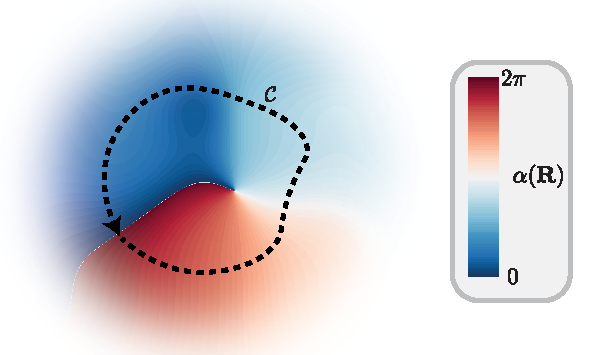
\includegraphics[]{local_markers_background/figures/branch cut.pdf}
    \caption[Colourmap of a local gauge transformation. ]{An example of a non-smooth gauge transformation designed to change the value of the Berry phase around the path $\mathcal C$ -- marked with a dashed line -- by an addition of $2\pi$. Only a small region of $\textbf R$-space is shown, with the local phase applied shown by the colourmap.}
    \label{fig:branch_cut}
    \end{center}
\end{figure}%
The exponential of the phase $e^{-i\gamma(\mathcal C)}$ around the loop \textit{is} gauge invariant, one can see this intuitively by realising that it is identical to the Berry phase from the discrete case, but in the limit where the discrete steps become arbitrarily close together. However, the Berry phase $\gamma(\mathcal C)$ itself is not strictly gauge invariant, since one can introduce a gauge transformation that creates a branch cut around the path $\mathcal C$. After traversing the whole path, the state at the end of the loop would have picked up a total phase $2\pi$, meaning that under a gauge transformation we can change the Berry phase according to 
\begin{align}
    \gamma (\mathcal C) \rightarrow \gamma (\mathcal C) + 
     2\pi n \textup{ for } n \in \mathbb Z.
\end{align}
An example of such a gauge transformation is shown in Fig.~\ref{fig:branch_cut}

\subsubsection{Berry Curvature}
Let us now define a quantity equivalent to the Berry flux from the previous discussion. Starting with Eqn.~\ref{eqn:flux_loop}, we use Stokes' theorem to transform it into a surface integral over a surface $\mathcal S$ bounded by the curve $\mathcal C$. We will consider the case for a two and three-dimensional parameter space $\mathcal R$, but of course this argument generalises to arbitrary dimensions.
\begin{align}
    \textup{In 2D: } & \gamma (\mathcal C) = \int_{\mathcal S} d^2R 
    \left ( 
        \partial_{x} A_{y}(\textbf R) - \partial_{y}A_{x}( \textbf R) 
    \right ) , \label{eqn:2d_berry_curvature} \\
    \textup{In 3D: } & \gamma (\mathcal C) = \int_{\mathcal S} d\textbf S \cdot 
    \left (
        \nabla_\textbf R \times \textbf{A}(\textbf R)
    \right ) ,  \label{eqn:3d_berry_curvature}
\end{align}
where we use the shorthand $\partial_\alpha = \frac{\partial}{\partial R_\alpha}$. Thus, we may define the Berry curvatures,
\begin{align}
    \Omega (\textbf R) &= \partial_{x} A_{y}( \textbf{k}) - \partial_{y}A_{x}( \textbf R) \\ 
    \bm \Omega( \textbf R) &= \nabla_\textbf R \times \textbf{A}(\textbf R).
\end{align}
 
\begin{shaded}
{\it Two Useful Ways to Re-express the Berry Curvature ---} Now let us focus only on the 2D case and reformulate this expression in two different ways.

\begin{enumerate}
    \item The first way finds the curvature in terms of the rate of change of the Hamiltonian only. Writing this quantity out explicitly in terms of the states $\ket{\psi(\textbf R)}$, we arrive at
    \begin{align}\label{berry_curvature_state_deriv}
        \Omega(\textbf R) = i \braket{  \partial_x \psi(\textbf R) | \partial_y \psi(\textbf R)} + h.c.
    \end{align}
    We can insert a resolution of the identity $\1 = \sum_n \ketbra{\psi_n}{\psi_n}$ to obtain
    \begin{align}
        \Omega(\textbf R) = i \sum_{\psi_n \neq \psi} \braket{  \partial_x \psi|\psi_n }\braket{ \psi_n|\partial_y \psi} + h.c.
    \end{align}
    Using the identity, 
    \begin{align}
        \braket{\psi_n | \partial_\alpha \psi} = \frac{
            \braket{\psi_n | \partial_\alpha H | \psi}
        }{
            \epsilon - \epsilon_n
        }, \ \textup{for } \psi \neq \psi_n,
    \end{align}
    we can re-express the Berry curvature in the form
    \begin{align} \label{eqn:berry_curvature_hamiltonian}
        \Omega(\textbf R) = i \sum_{\psi_n \neq \psi} 
        \frac{
            \braket{ \psi|\partial_x H|\psi_n }\braket{ \psi_n| \partial_y H |\psi}
        }{
            (\epsilon - \epsilon_n)^2
        } + h.c.
    \end{align}

    \item Note that the definition provided for the Berry curvature  (Eqn.~\ref{berry_curvature_state_deriv}) is only well-defined across $\mathcal R$ when the state remains fully gapped. That is, no other states ever have the same energy as $\ket{\psi(\textbf R)}$. When another state's energy crosses that of $\ket \psi$, the individual states become ill-defined and so it becomes challenging to write down a natural derivative for the states. With this in mind, let us consider re-expressing the Berry curvature in terms of the single state projector $\hat \psi = \ketbra\psi \psi$,
    \begin{align} \label{eqn:operator_berry_curvature}
        i \braket{  \partial_x \psi | \partial_y \psi} + h.c.
        =
        i \tr \left [ \hat \psi \partial_x \hat \psi \, \partial _y \hat \psi \right ] + h.c.
    \end{align} 
    For a single state, this is identical to the regular Berry curvature, however the utility of this expression becomes evident when we construct it for a projector onto a set of states $P = \sum_{i \in \textup{band}} \ketbra {\psi_i}{\psi_i} $. Since $\partial P$ is still well-defined when the states in $P$ are degenerate, we can write an expression for the combined Berry curvature of a set of states that can handle degeneracy (provided no states outside $P$ become degenerate with $P$).
    \begin{align}
        \Omega_P = i\tr \left [ P \partial_x P \partial_y P \right ] + h.c.
    \end{align}
\end{enumerate}
\end{shaded}

This calculation has one important caveat. It is only possible to apply Stokes' theorem when $\textbf A$ is smooth over the region $\mathcal{R}$. This means that we need to have already picked a smooth gauge in the region we are integrating over to have a guarantee that Eqns.~\ref{eqn:2d_berry_curvature} and \ref{eqn:3d_berry_curvature} hold. If we transform to a non-smooth gauge then it is possible that the Berry phase will change by a multiple of $2\pi$, however the Berry curvature is truly gauge invariant. This can be seen from Eqn.~\ref{eqn:berry_curvature_hamiltonian}, where the Berry curvature is defined without the differentiation of states, so is invariant under even a non-smooth gauge transformation. Thus in general we only have the guarantee that
\begin{align}\label{eqn:berry_loop_to_curvature}
    e^{-i\gamma(\mathcal C)} = e^{\int_{\mathcal S} d^2 R\,  \Omega (\textbf R)}.
\end{align}
\subsubsection{Chern Number}

As in \textsection\ref{sec:discrete_chern}, we make the assertion that the manifold parametrised $\textbf R$ is closed, generally one is working on the torus. The Chern number can then be defined as the integral of the Berry curvature across the whole manifold,
\begin{align} \label{eqn:cont_chern_number}
    \mathcal Q &= \frac{1}{2\pi} \int d^2 R \, \Omega.
\end{align}
As in the discrete case, the Chern number is restricted to only take integer values. The argument follows the same lines as previously, where we can use our modified form of Stokes' theorem (Eqn.~\ref{eqn:berry_loop_to_curvature}). Since the manifold is close, it has no boundary, so the flux integral equivalent to the Berry phase around a loop enclosing no area, implying that
\begin{align}
    e^{\int d^R k\,  \Omega (\textbf R)} &= 1,
    \implies \mathcal Q \in \mathbb Z
\end{align}

\subsection{An Example -- The Two-Level System} \label{sec:an_example}

Let us illustrate these concepts with the example of a two-state system. Our first step is to parametrise the possible Hamiltonians in such a system using a vector $\textbf d$. We will then solve this Hamiltonian for the positive and negative energy eigenstates. This allows us to look at how the eigenstates change as we smoothly deform the Hamiltonian, exploring the parameter space. By examining how the eigenstates of $\hat H$ depend on $\textbf d$, we can calculate the Berry curvature of the positive and negative energy states. We then connect this with our understanding of the Bloch states in a periodic quantum system. We discuss how the bulk Hamiltonian of a periodic system corresponds to the embedding of a closed surface in $\textbf d$-space and describe how to calculate the Chern number of the bands in such a system.

The Hilbert space of a two-level system is given by rays in $\mathbb C ^2$. Any Hamiltonian acting on this space must be a $2\times 2$ Hermitian matrix, which we parametrise in terms of a Pauli vector $\textbf d$,
\begin{align}
    H = \textbf{d}\cdot\hat{\sigma}  = d_i \sigma^i,
\end{align}
where the $\sigma^i$ are the Pauli matrices. This gives us a complete basis for $2\times2$ traceless Hermitian matrices. Of course, we could include a multiple of the identity to span the full space of Hermitian matrices, however this would have no effect on the topology, and shall be omitted.

The set of traceless Hamiltonians is thus a manifold in itself, $ \{H\} \cong \mathbb{R}^3 $, since $\textbf{d} \in \mathbb{R}^3 $. Here we shall restrict to gapped Hamiltonians, so $\textbf d = 0$ is forbidden, leaving $ \{H\} \cong \mathbb{R}^3\backslash 0$. The first thing we will do is to express the vector $\textbf{d}$ in spherical polar coordinates,
\begin{align}
    H = |\textbf{d}|\begin{pmatrix}
\cos(\theta) &e^{-i\phi}\sin{\theta} \\ 
 e^{i\phi}\sin{\theta}& -\cos(\theta)
\end{pmatrix}
\end{align}
This matrix has $H^2 = |\textbf{d}|^2 \1 $, so its eigenvalues are $\pm |\textbf{d}|$, with eigenvectors
\begin{align}\label{states}
    \ket{+_{\textbf{d}}} = \begin{pmatrix}
e^{-i\phi/2}\cos(\theta/2)\\ 
e^{i\phi/2} \sin(\theta/2)
\end{pmatrix},\; \ket{-_{\textbf{d}}} = \begin{pmatrix}
-e^{-i\phi/2}\sin(\theta/2)\\ 
e^{i\phi/2} \cos(\theta/2)
\end{pmatrix}.
\end{align}
We have thus arrived at a set of states, $\ket {\pm_{\textbf d}}$ that depend on the parameter $\textbf d$, meaning we can apply the techniques of the last section. From Eqns.~\ref{eqn:cont_berry_connection} and \ref{eqn:3d_berry_curvature} we know that the Berry connection and Berry curvature of the $\ket \pm$ states are given by
\begin{align}
    \textbf{A}^\pm (\textbf d) &= i\braket{\pm_\textbf{d} | \nabla_\textbf{d}| \pm_\textbf{d}}\\
    \bm \Omega^{\pm}(\textbf d ) &= \nabla_\textbf{d} \wedge \textbf{A}^\pm (\textbf d).
\end{align}
Using this equation it is possible to directly calculate the Berry curvature, arriving at the following expression:
\begin{align}
    \bm \Omega^{\pm} = \pm \frac{\hat{n}_\textbf{d}}{2\textbf{d}^2}
\end{align}
where $\hat{n}_\textbf{d}$ is a unit vector pointing parallel to $\textbf{d}$.

This Berry curvature is equivalent to a monopole field radiating out from the origin in $\textbf d$-space, in analogy with electrostatics. Thus, the Berry phase of the $\ket{+_{\textbf d}}$ state around some path in $\textbf d$-space is given by
\begin{align}
	\gamma^+ (C) = \oint_{\mathcal C} \textbf A^+ (\textbf d) \cdot d \textbf d.
\end{align}
Re-expressing this in terms of the Berry curvature gives us
\begin{align}
	\gamma^+ (C) = \int_{\mathcal R} \bm \Omega^+ (\textbf d) \cdot d \textbf S,
\end{align}
where the integral is over a region $\mathcal R$ that has the curve $\mathcal C$ as its boundary. Since the Berry curvature is just a monopole field with charge $\frac{1}{2}$, this integral ends up evaluating half the solid angle subtended by the curve $\mathcal C$.
% \begin{equation}
%     \gamma^+ (C) = \frac{1}{2}\Omega_{\mathcal{C}}.
% \end{equation}

\subsubsection{Chern Number}
Now we can connect this with our understanding of Bloch states. For a two-dimensional translationally symmetric system, the Hamiltonian can be diagonalised according to
\begin{align}
	 H = \sum_{\textbf k} \ket{\textbf k}\bra{\textbf k} \otimes  H (\textbf k).
\end{align}
If the unit cell contains two sites, then $ H (\textbf k)$ is a $2 \times 2$ matrix that depends on $\textbf k$. We can write it in terms of a $\textbf d$ vector that depends on $\textbf k$.
\begin{align}
H(\textbf{k}) &= \textbf{d}(\textbf{k})\cdot {\sigma}.
\end{align}
Here, $\textbf{k}$ lives on the surface of a torus, since $k_x$ and $k_y$ are periodic. Furthermore, $\textbf{d}$ (and by extension $ H$) live in the space $\mathbb{R}^3\backslash 0$. Thus, $\textbf{d} ( \textbf k )$ is a map of the form
\begin{align}
    \textbf{d} : S^1 \times S^1 &\rightarrow \mathbb{R}^3\backslash 0 .
\end{align}
The map is an embedding of a two-dimensional surface (the torus) into three-dimensional flat space ($\mathbb{R}^3$). The only constraint placed on this map is that it must remain smooth, however the embedded torus can take any shape.

To calculate the Berry phase around a loop in k-space, all we have to do is look at the corresponding loop in d-space. Then we integrate the Berry connection over some surface that has this loop as its boundary. Since the Berry curvature has the form of a monopole flux, we can simplify further -- one must simply find the solid angle subtended by the curve around the origin and divide it by two.

\begin{center}
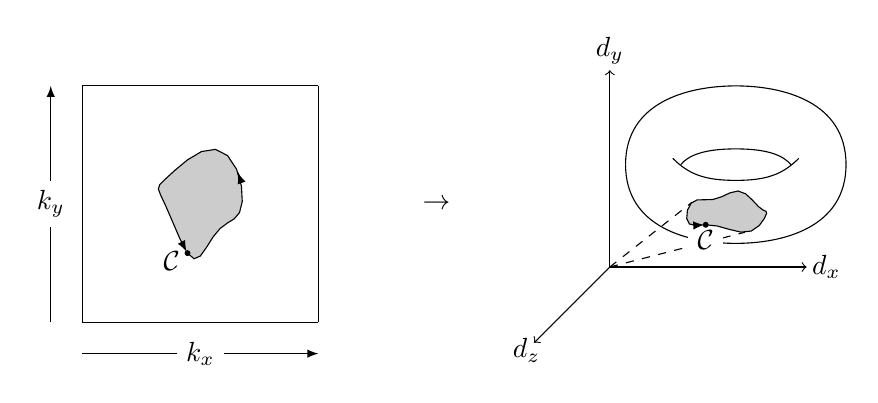
\begin{tikzpicture}

\def \axissize {2.5}
\def \squaresize{1.5}

\def \squarepos{-3}
\def \axisxpos {2.2}
\def \axisypos{-0.8}
\def \arrowdistance {0.4}

\draw (\squarepos - \squaresize , - \squaresize) -- (\squarepos + \squaresize, - \squaresize);
\draw (\squarepos + \squaresize , - \squaresize) -- (\squarepos + \squaresize, + \squaresize);
\draw (\squarepos + \squaresize , + \squaresize) -- (\squarepos - \squaresize, + \squaresize);
\draw (\squarepos - \squaresize , + \squaresize) -- (\squarepos - \squaresize, - \squaresize);

\draw [-latex] (\squarepos - \squaresize  , - \squaresize-\arrowdistance) -- (\squarepos + \squaresize, - \squaresize- \arrowdistance);
\draw [-latex] (\squarepos - \squaresize-\arrowdistance, - \squaresize) -- (\squarepos - \squaresize -\arrowdistance, + \squaresize) ;

\draw node [fill= white] at (\squarepos  , - \squaresize-\arrowdistance) {$k_x$};
\draw node [fill= white] at (\squarepos - \squaresize-\arrowdistance, 0)  {$k_y$};

\draw [-latex, fill= black!20, domain = 0:358] plot ({0.5 * (cos(\x-120) + 0.2 * sin(2*(\x-120))) + \squarepos},{0.6*(sin(\x-120) + 0.2 * cos(3*(\x-190))) });
\draw [-latex, domain = 160:161] plot ({0.5 * (cos(\x-120) + 0.2 * sin(2*(\x-120))) + \squarepos},{0.6*(sin(\x-120) + 0.2 * cos(3*(\x-190))) });

\draw[fill] ({0.5 * (cos(-120) + 0.2 * sin(2*(0-120))) + \squarepos},{0.6*(sin(-120) + 0.2 * cos(3*(-190))) }) circle [radius=0.03];
\draw node at ({0.5 * (cos(-120) + 0.2 * sin(2*(0-120))) + \squarepos -0.2 },{0.6*(sin(-120) + 0.2 * cos(3*(-190))) -0.1 }) {$\mathcal C$};


\draw node at (0,0) {$ \rightarrow$};

\draw [->] (\axisxpos,\axisypos,0) -- (\axisxpos+\axissize,\axisypos,0);
\draw  [->] (\axisxpos,\axisypos,0) -- (\axisxpos,\axisypos+\axissize,0);
\draw  [->] (\axisxpos,\axisypos,0) -- (\axisxpos,\axisypos,\axissize);

\def \donutscale {0.4}
\def \donutx {3.8}
\def \donuty {0.5}

\draw (-3.5*\donutscale+\donutx,0+\donuty) .. controls (-3.5*\donutscale+\donutx,2*\donutscale+\donuty) and (-1.5*\donutscale+\donutx,2.5*\donutscale+\donuty) .. (0+\donutx,2.5*\donutscale+\donuty);
\draw[xscale=-1] (-3.5*\donutscale-\donutx,0+\donuty) .. controls (-3.5*\donutscale-\donutx,2*\donutscale+\donuty) and (-1.5*\donutscale-\donutx,2.5*\donutscale+\donuty) .. (0-\donutx,2.5*\donutscale+\donuty);
\draw[rotate=180] (-3.5*\donutscale-\donutx,0-\donuty) .. controls (-3.5*\donutscale-\donutx,2*\donutscale-\donuty) and (-1.5*\donutscale-\donutx,2.5*\donutscale-\donuty) .. (0-\donutx,2.5*\donutscale-\donuty);
\draw[yscale=-1] (-3.5*\donutscale+\donutx,0-\donuty) .. controls (-3.5*\donutscale+\donutx,2*\donutscale-\donuty) and (-1.5*\donutscale+\donutx,2.5*\donutscale-\donuty) .. (0+\donutx,2.5*\donutscale-\donuty);
\draw (-2*\donutscale+\donutx,.2*\donutscale+\donuty) .. controls (-1.5*\donutscale+\donutx,-0.3*\donutscale+\donuty) and (-1*\donutscale+\donutx,-0.5*\donutscale+\donuty) .. (0+\donutx,-.5*\donutscale+\donuty) .. controls (1*\donutscale+\donutx,-0.5*\donutscale+\donuty) and (1.5*\donutscale+\donutx,-0.3*\donutscale+\donuty) .. (2*\donutscale+\donutx,0.2*\donutscale+\donuty);
\draw (-1.75*\donutscale+\donutx,0+\donuty) .. controls (-1.5*\donutscale+\donutx,0.3*\donutscale+\donuty) and (-1*\donutscale+\donutx,0.5*\donutscale+\donuty) .. (0+\donutx,.5*\donutscale+\donuty) .. controls (1*\donutscale+\donutx,0.5*\donutscale+\donuty) and (1.5*\donutscale+\donutx,0.3*\donutscale+\donuty) .. (1.75*\donutscale+\donutx,0+\donuty);

\def\spposx{3.7}
\def\spposy{-0.1}

\def \angone {280}
\def \angtwo {50}

\draw [dashed] (\axisxpos,\axisypos,0) -- ({0.5 * (cos(\angone-120) + 0.1 * sin(2*(\angone-20))) + \spposx},{0.23*(sin(\angone-120) + 0.2 * cos(4*(\angone-190))) +\spposy});
\draw [dashed]  (\axisxpos,\axisypos,0) -- ({0.5 * (cos(\angtwo-120) + 0.1 * sin(2*(\angtwo-20))) + \spposx},{0.23*(sin(\angtwo-120) + 0.2 * cos(4*(\angtwo-190))) +\spposy});

\draw  node [fill=white]  at ({0.5 * (cos(-120) + 0.1 * sin(2*(-20))) + \spposx},{0.23*(sin(-120) + 0.2 * cos(4*(-190))) +\spposy-0.2}) {$\mathcal C$};

\draw [-latex, fill= black!20, domain = 0:358] plot ({0.5 * (cos(\x-120) + 0.1 * sin(2*(\x-20))) + \spposx},{0.23*(sin(\x-120) + 0.2 * cos(4*(\x-190))) +\spposy});
\draw[fill] ({0.5 * (cos(-120) + 0.1 * sin(2*(-20))) + \spposx},{0.23*(sin(-120) + 0.2 * cos(4*(-190))) +\spposy}) circle [radius=0.03];


\draw node at (\axisxpos+1.1*\axissize,\axisypos,0){$ d_x$};
\draw  node at  (\axisxpos,\axisypos+ 1.1*\axissize,0){$ d_y$};
\draw  node at (\axisxpos,\axisypos, 1.1*\axissize){$d_z$};
\end{tikzpicture}
\end{center}

What about the Chern number? This is found by the integrating the Berry curvature across the whole surface of the torus in d-space. If the embedding of the torus does not contain the origin, then the value of this integral is necessarily zero. Now suppose the torus is embedded such that it contains the origin, then we will have a surface that catches all the Berry flux on its inside and the solid angle subtended is $4\pi$. Thus, the Chern number is $+1$. Similarly, for an embedding that wraps the torus twice around the origin, the subtended flux will correspond to twice the charge of the monopole, leading to a Chern number of $+2$. Thus, we see that the Chern number in this context must be quantised, and can often be read directly from the form of $\textbf d(\textbf k)$ by asking how many times this embedding of the torus wraps the origin.

\subsection{Final Notes}

We close this section with an explanation of the consequences of Chern number in topological insulators.

\subsubsection{Smoothly Deforming the Hamiltonian}

Consider a pair of quantum systems in the same Hilbert space, described by Hamiltonians $\hat H_1$ and $\hat H_2$ which are both gapped at the Fermi level. We might ask: \textit{Is it possible to smoothly deform $\hat H _1$ into $\hat H_2$ without crossing a point where the gap at the Fermi level closes?}

The answer is that it is only possible if the sum of the Chern numbers of the occupied bands of $\hat H_1$ and $\hat H_2$ are the same. This is because the total Chern number of the occupied bands is restricted to only take integer values -- it cannot smoothly change as we deform the Hamiltonian. For the total Chern number to change, we must somewhere cross a point where it is impossible to define a Chern number at all, allowing it to jump discontinuously when we leave that point. This is precisely what happens when the gap at the Fermi level closes. At this point, the occupied bands can no longer be defined as a smooth object in momentum space, since there must be a discontinuity at the band touching point. 

We can illustrate this with the example in \textsection\ref{sec:an_example}. Smoothly deforming the Hamiltonian amounts to changing the shape of the torus embedded in $\textbf d$-space. If any point on the surface of the torus touches the origin, a pair of zero-energy states must appear -- the gap has closed, and the system is conductive. If the band has a Chern number of $+1$, this means that the torus contains the origin. In order to smoothly deform this into a system with zero Chern number, we would need to move the torus such that the origin was now outside. At some point in this deformation the torus surface will have to pass through the origin, creating a conducting Hamiltonian at that point.

Thus, we can classify all Hamiltonians according to the Chern number of their bands. It is always impossible to smoothly deform a Hamiltonian into one with a different Chern number while remaining insulating. Similarly, it is always possible to smoothly deform two Hamiltonians into one another without closing a gap, provided that their bands have identical Chern numbers\footnote{A simple justification for this comes from band flattening. Any Hamiltonian can be smoothly band flattened, where all the states in each band are set to the same energy. Furthermore, for a given set of Chern numbers, all band flattened Hamiltonians (with the same dimensionality) are equivalent. Thus, any two Hamiltonians with identical Chern numbers can be transformed into one another by using the common band flattened Hamiltonian as an intermediate step.}~\cite{avron_homotopy_1983}.

\subsubsection{The Bulk-Boundary Correspondence}

The argument presented above allows us to make a rough justification for why conducting edge states must appear wherever we have a material with nonzero Chern number. Suppose we have a large system where the Hamiltonian is allowed to vary slowly over space, defined by $\hat H (\textbf r)$. In one region this Hamiltonian locally has non-zero Chern number, $\hat H _{\textup{topological}}$, but in a different distant region it locally has zero Chern number, $\hat H _{\textup{trivial}}$. We expect that between these regions the Hamiltonian must be gradually transforming between $\hat H _{\textup{topological}}$ and $\hat H _{\textup{trivial}}$. As we have seen, it is impossible for our Hamiltonian to make this transformation without passing through a conducting region somewhere along the way -- edge states must appear! Exploiting this intuition, one might view the vacuum as having zero Chern number. Thus, we would expect that if a material with non-zero Chern number transforms over space into the vacuum -- that is, it has a boundary -- then conductive states must appear at the boundary. This property of Chern insulators is called the bulk-boundary correspondence \cite{qi_general_2006,hasan_colloquium_2010,qi_topological_2011}.


\subsubsection{Chern Number and Globally Smooth Gauges}\label{sec:chern_smooth_gauge}
Carefully considering the gauge used in Eqn.~\ref{states}, one might notice that there is a discontinuity at $\phi = \pi$ where $e^{i\phi}$ suddenly jumps as you cross over to $\phi = -\pi$. This is no oversight, it is completely impossible to define a globally smooth set of states $\ket{\psi(\textbf{d})}$ for any band that has nonzero Chern number. This is because if $\ket{\psi(\textbf{d})}$ were continuous everywhere, then the Berry connection would also have to be continuous everywhere. Thus, we could invoke Stokes' theorem in Eqn.~\ref{eqn:cont_chern_number}, showing that the Chern number must vanish since the integral is over the whole (closed) manifold. A nonzero Chern number thus relies on there being points where Stokes' theorem cannot be used. In this sense, the Chern number can be regarded as a measure of the amount of discontinuity that \textit{must} be present regardless of the gauge you choose for the space.




\section{The QWZ Model and its Amorphous Counterpart}
For the rest of this document, we will use the Qi-Wu-Zhang (QWZ) model as our example for a topological insulator, first introduced in \cite{qi_topological_2006}. This is because the QWZ model is a simple toy model for a two-dimensional topological insulator with nearest-neighbour interactions on a square lattice.\par
 We work in a similar Hilbert space as that used in \textsection\ref{sec:lattice_bloch}, on a lattice of unit cells indexed by a two dimensional lattice vector $\bf m$, where each cell contains two sites -- the QWZ model has two bands. Thus the Hilbert space of the system is spanned by states of the form
\begin{align}
    \ket{\psi} = \ket{m_x} \otimes \ket{m_y} \otimes \ket{\alpha}.
\end{align}
The lattice has size $(L_x,L_y)$, so we have 
\begin{align}
    m_x \in \{ 0,...,L_x-1\}\\
    m_y \in \{ 0,...,L_y-1\}\\
    \alpha \in \{0,1\}.
\end{align}
The QWZ model is defined by three terms, a hopping between unit cells in the $x$-direction, a hopping in the $y$-direction, and a staggered on-site potential whose strength is determined by a parameter $u$.
\begin{align}
    \hat H &= \sum_{\bf m} \ket{\bf m+ 1_x}\bra{\bf m} \otimes \frac{\sigma_z + i\sigma_x}{2} + h.c. \nonumber \\
    &+ \sum_{\bf m} \ket{\bf m+ 1_y}\bra{\bf m} \otimes \frac{\sigma_z + i\sigma_y}{2} + h.c. \nonumber \\
    &+ \sum_{\bf m} \ket{\bf m}\bra{\bf m} \otimes u\; \sigma_z,
\end{align}
where $1_x$ and $1_y$ represent the unit displacement in their respective directions,
\begin{align}
	1_x = \begin{pmatrix}
	1\\
	0
	\end{pmatrix}, \ 1_y = \begin{pmatrix}
	0\\
	1
	\end{pmatrix}.
\end{align}
\begin{figure}[t]
\begin{center}
 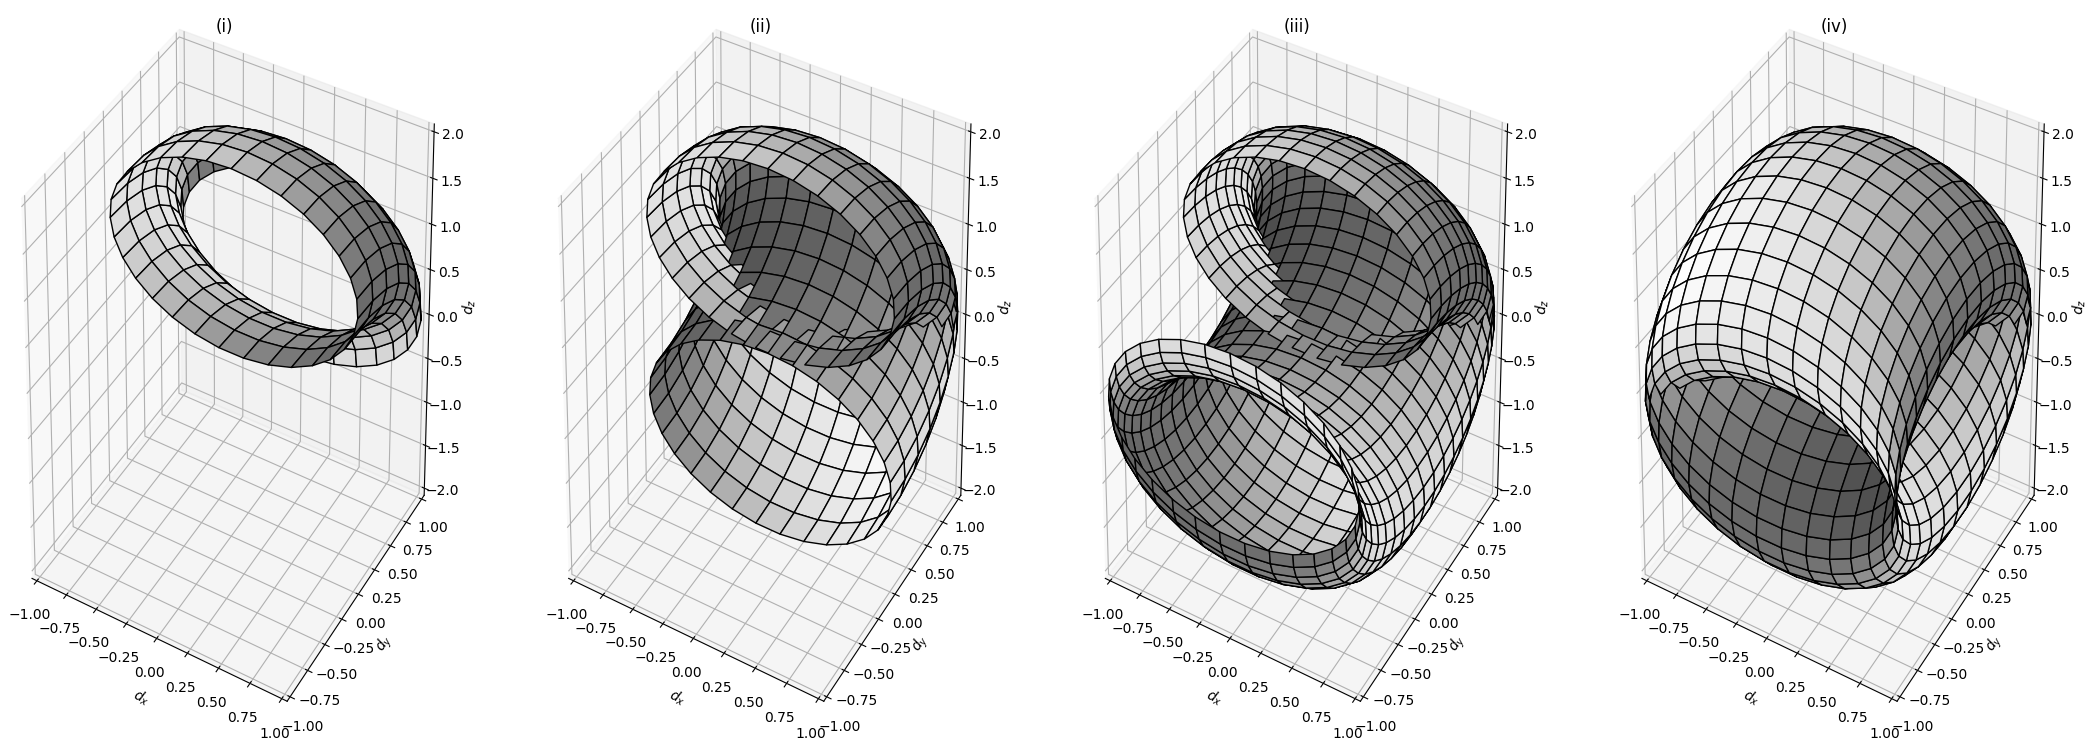
\includegraphics[width=\textwidth]{local_markers_background/figures/QWZ_donut.png}
\caption{The embedding of the Brillouin zone in $\bf d$-space for the QWZ model. This is shown in four progressive cutaways to ensure the internal structure can be seen. In all four images $k_x$ spans the interval $\left ( 0, 2\pi \right ]$, however in (i) $k_y$ spans $\left ( 0, \frac{\pi}{2} \right ]$, in (ii) $k_y$ spans $\left ( 0, \pi \right ]$, in (iii) $k_y$ spans $\left ( 0, \frac{3 \pi}{2} \right ]$, and in (iv) $k_y$ spans $\left ( 0, 2\pi \right ]$. }
\label{fig:QWZ_donut}
\end{center}
\end{figure}
Using Bloch's theorem, we can find the bulk Hamiltonian,
\begin{align}
    \hat H(\bf k) = \begin{pmatrix}
\sin k_x \\ 
\sin k_y\\ 
u + \cos k_x+ \cos k_y
\end{pmatrix} \cdot \bm \sigma.
\end{align}
Here, $k_x$ and $k_y$ determine our position in the Brillouin zone. As explained in \textsection\ref{sec:an_example}, this represents the embedding of a torus in $\bf d$-space, shown in fig. \ref{fig:QWZ_donut}.\par
The $u$-parameter has the effect of translating the torus by a fixed amount in the $z$-direction. From this we can see that the QWZ model only has non-zero Chern number for values of $u$ between -2 and 2. This is because translating the torus by any more than this will place the origin completely outside. The Chern number for the QWZ model is
\begin{align}
Q = \left\{\begin{matrix}
-1 &:&  -2 < u < 0 \\ 
1  &:&  0<u<2\\
0  &:&  \textit{otherwise} 
\end{matrix}\right. ,
\end{align}
not including the points at $u =$ -2, 0 and 2, at which the Chern number is undefined because the band gap closes and the material is conducting. Some example band structures for varying values of $u$ are shown in fig. \ref{fig:QWZ_band_struct}.
\begin{figure}[t]
\begin{center}
 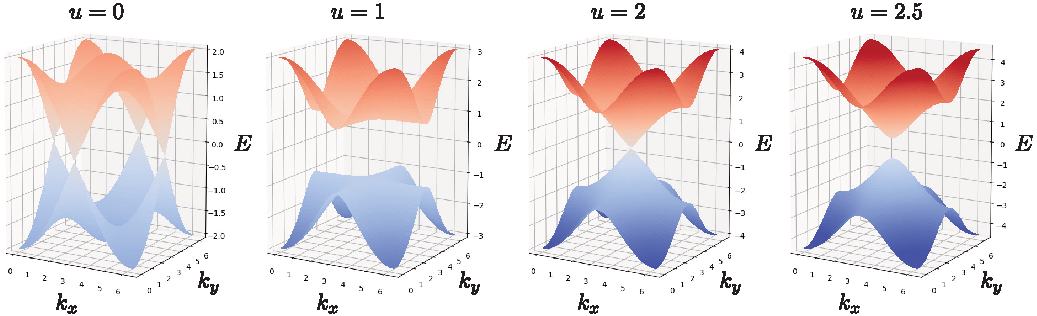
\includegraphics[width=\textwidth]{local_markers_background/figures/QWZ_band_struct}
\caption{Four examples of the band structure of the QWZ model are shown, for varying $u$ values between 0 and 2.5. At $u$ = 0 and 2, the bands touch and Chern number is undefined. At $u$ = 1, Q = +1, and at $u$ = 2.5, Q = 0.}
\label{fig:QWZ_band_struct}
\end{center}
\end{figure}

\subsection{Strip Geometry} \label{sec:QWZ_strip_geometry}
In much of the following discussion, we will be studying the QWZ model in a system with strip geometry. This means that the lattice is periodic and uniform in the $y$-direction, but is allowed to be non-uniform or have open boundaries in the $x$-direction. We will allow $u$ to vary in the $x$-direction, so add a subscript to indicate position-dependence $u \rightarrow u_{m_x}$. We can apply Bloch's theorem in the $y$-direction only, and our eigenstates take the following form,
\begin{align}
    \ket{\psi} = \ket{k_y}\otimes \ket{v_{k_y}^{n,l}},
\end{align}
where $\ket{k_y}$ is a plane wave solution
\begin{align}
    \ket{k_y} =\frac{1}{\sqrt{L_y}} \sum_{m_y} e^{i m_y k_y}\ket{m_y},
\end{align}
and $\ket{v_{k_y}^{n,l}}$ is a $2L_x$-element vector in the remaining part of the Hilbert space $\mathcal H_x \otimes \mathcal H_{\textup{int}} $. The $n$ index labels which band the state is in, and the $l$ index differentiates between the states in each band.
\begin{align}
    n &\in \{0,1\}\\
    l &\in \{ 0, \dots ,L_x -1\}.
\end{align}
The $v$-states are solutions of the semi-bulk Hamiltonian
\begin{align}
    \hat H(k_y) &= \sum_{m_x} \ket{m_x+1}\bra{m_x} \otimes \frac{\sigma_z + i\sigma_x}{2} + h.c.\nonumber \\
    &+ \sum_{m_x} \ket{m_x}\bra{m_x} \otimes \left [ (u_{m_x} + \cos k_y) \; \sigma_z + \sin k_y \; \sigma_y  \right ].
\end{align}
We have effectively reduced our system from a lattice of interacting sites in $x$ and $y$, to a set of chain models in $x$, that are each labelled by a value of $k_y$.
\begin{center}
\input{local_markers_background/figures/lattice_to_chain}
\end{center}
We can rewrite this, in terms of the $2\times2$ matrices $A$ and $B$,
\begin{align}
    A &= (u + \cos k_y) \; \sigma_z + \sin k_y \; \sigma_y,  \\ 
    B &= \frac{\sigma_z + i\sigma_x}{2},
\end{align}
and express our wavevectors in terms of a set of $L_x$ two-element states $\psi_n$
\begin{align}
    \ket{\psi} = \begin{pmatrix}
    \psi_0 \\
    \psi_1 \\
    \vdots \\
    \psi_{L_x -1}
     \end{pmatrix},
\end{align}
to arrive at a set of equations for the eigenvalues of the semi-bulk Hamiltonian.
\begin{align}
    \textup{Bulk:} &\ A\psi_n + B\psi_{n+1} + B^\dag \psi_{n-1} = \lambda \psi_n \\
    \textup{Left Edge:} &\ A\psi_1 + B\psi_{2} = \lambda \psi_1\\
    \textup{Right Edge:} &\ A\psi_{L_x} + B^\dag \psi_{L_x-1}  = \lambda \psi_n
\end{align}
The band structure for this system in both periodic boundaries and strip geometry is shown in fig. \ref{fig:strip_energy}.
\begin{figure}[t]
\begin{center}
 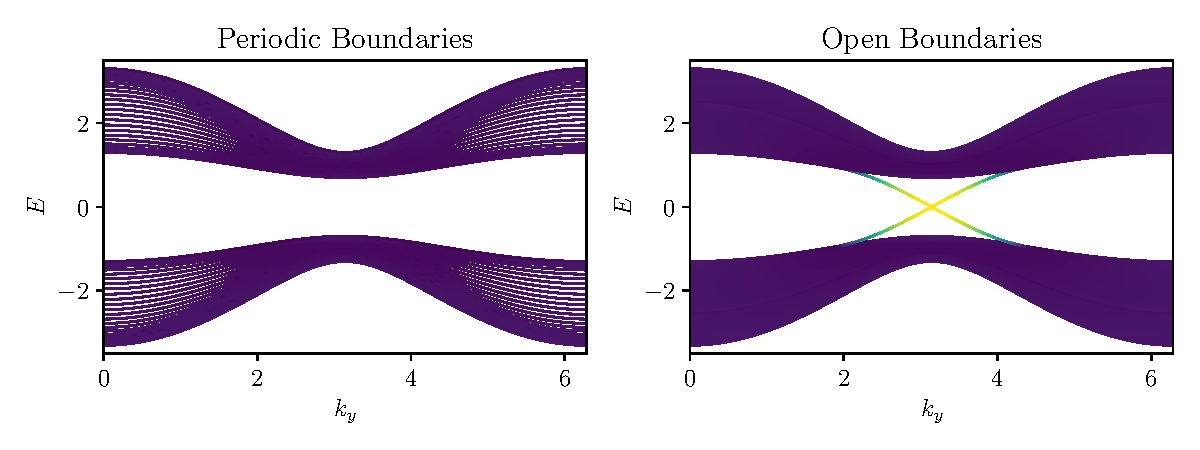
\includegraphics[width=.85\textwidth]{local_markers_background/figures/strip_energy}
\caption{An example band structure for a QWZ model with $u$ = 1.3 and $L_x$ = 30. On the left is the example for periodic boundary conditions, showing two well-separated bands. On the right is the case for open boundary conditions. Two edge states are shown leaving the bulk and crossing the gap, with the descending state being a left edge state, and the ascending state being a right edge state. }
\label{fig:strip_energy}
\end{center}
\end{figure}
We can now look at solving this analytically for the bulk and edge states. We will omit this calculation and print only the form of the results, however a full derivation can be found in appendix \ref{sec:QWZ_model_appendix}. Note that edge states are only present for certain values of $k_y$, which can be seen in figure \ref{fig:strip_energy}, where the edge states only separate from the bulk in a region around $k_y = \pi$. \par
Edge states have the form
\begin{align}
    \ket{\psi^{\textup{left}}_{k_y}} = \sqrt{1-\xi_l^2}\sum_{m=1}^{L_x} \xi_l^{m-1}\ket m \otimes \begin{pmatrix}
    1\\
    -i
    \end{pmatrix}
\end{align}
where 
\begin{align}
    \xi_l &= -u - \cos k_y.
\end{align}
This state has energy
\begin{align}
    E_l &= -\sin k_y.
\end{align}
Similarly, the right edge state is given by
\begin{align}
    \ket {\psi^{\textup{right}}_{k_y}} = \sqrt{1-\xi_r^2} \sum_{m=1}^{L_x} \xi_r^{L_x-m} \ket m \otimes  \begin{pmatrix}
    1\\
    i
    \end{pmatrix}
\end{align}
with the extra conditions
\begin{align}
   	 \xi_r &= -u-\cos k \label{eqn:edge_condition}\\
	E_r &= \sin k.
\end{align}
These edge states are only valid solutions for $k_y$ in the region
\begin{align}
	-1 < u+\cos k_y < 1.
\end{align}
These limits can be seen in fig. \ref{fig:strip_energy}, where the edge states peel away from the bands to cross the energy gap.\par
The bulk states are less straightforward to obtain exact solutions for, we give the general form for them and leave the details to appendix \ref{sec:QWZ_model_appendix}.
\begin{align}
    \ket{\psi^\pm_{k_y} }= \frac{1}{\sqrt{L_x}}\sum \ket{m}  \otimes \left [ \alpha e^{i \theta m} \ket{\phi_{\theta}^{\pm}} + \beta e^{-i \theta m} \ket{\phi_{\theta}^{\pm *}} \right ],
\end{align}
where the exact values of $\theta$, $\alpha$, $\beta$ and $\ket{\phi_{\theta}^{\pm}} $ can be found by solving some fairly unpleasant equations.\par
Here we mention a final caveat, These calculations are only strictly valid in the limit of a large system. This is because we have made the assumption the edge states can be calculated by taking into consideration only one edge and ignoring the effect of the other. The edge states decay exponentially through the system, so we are relying on the assumption that the edge state has effectively decayed to nothing before reaching the other side. When this condition is relaxed the edge states are able to couple to one another. This has a two effects, the first being that at the crossing of edge states, our energy eigenvalues become positive and negative superposition states of both edge states. The other is that the left state coupling to the right state shifts their energy levels such that no states cross $E = 0$ -- there is no longer a crossing of energy levels for the left and right edge states.




\subsection{The Amorphous QWZ Model}


\section{Local Markers}
\subsection{Kitaev's Local Marker}

\subsection{The Bott Index}

\subsection{The Chern Marker}

\bibliographystyle{unsrt}
\bibliography{local_markers/local_markers.bib}